\documentclass[12pt,a4paper,oneside]{article}

\usepackage[left=1.5cm, right=1cm, top=1cm, bottom=1.5cm]{geometry}

\usepackage[utf8]{inputenc}
\usepackage[T2A]{fontenc}
\usepackage[english, russian]{babel}

\usepackage{graphicx}
\usepackage{wrapfig}
\graphicspath{ {./} }

\title{\textbf{Инструкция по сборке}}
\author{Дельта Альфа Альфа Штрих}
\date{}

\begin{document}

\maketitle

\noindent\rule{\textwidth}{1pt}

\begin{flushright}
    \textit{Штрилиц постучал в дверь 5 раз, дверь постучала в Штирлица 5 раз.\\
        — Третий закон Ньютона, — подумал Штирлиц.}
\end{flushright}

% \begin{wrapfigure}{r}{\textwidth} \centering
%     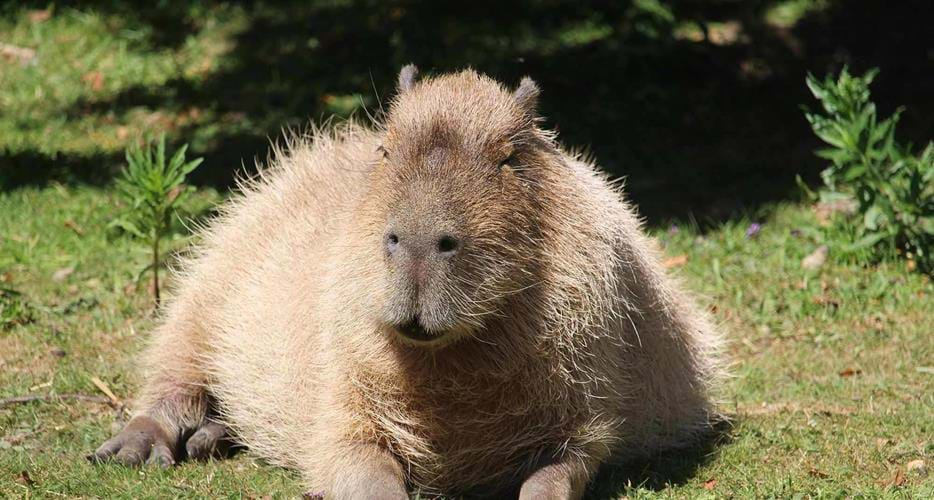
\includegraphics[width=\textwidth]{capybara} \end{wrapfigure}

\section{Сборка верхней панели с кнопкой}
Установить TopPanel наверх и закрепить её DIN7985-M4 винтами с T гайками.
Вставить кнопку в круглое отверстие для кнопки.

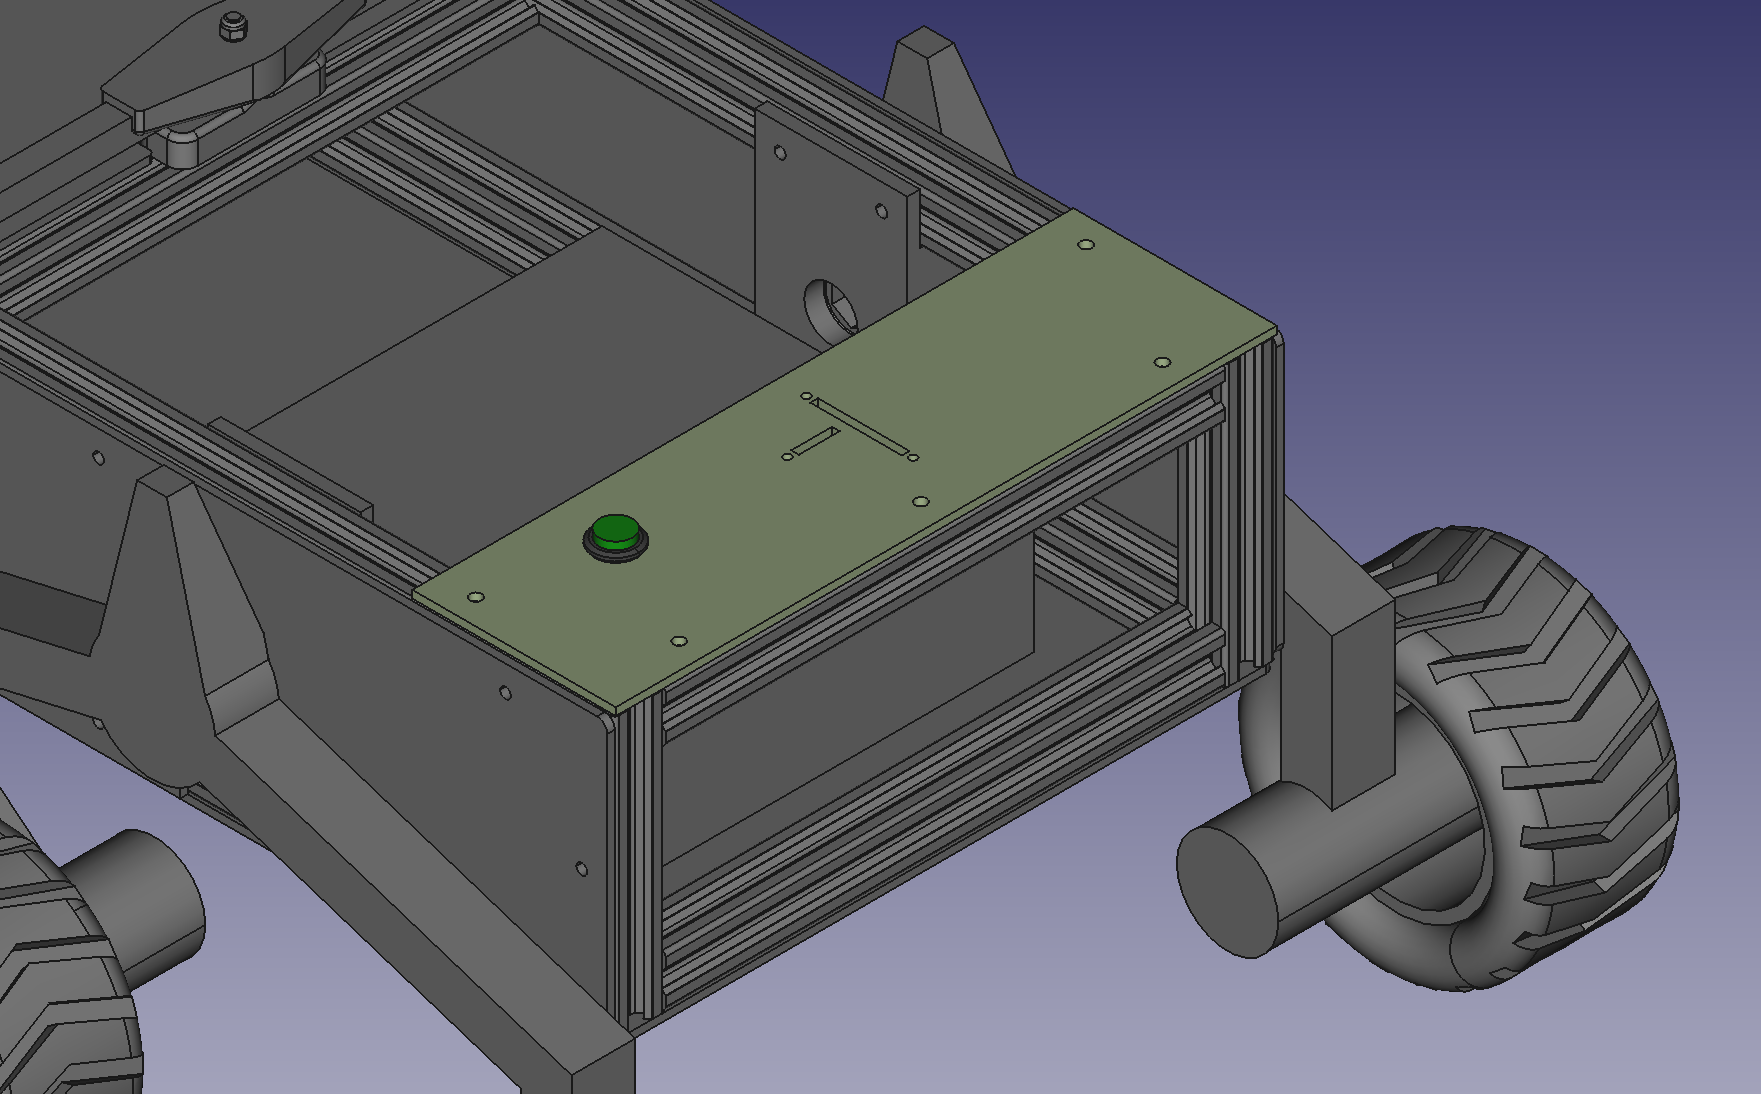
\includegraphics[width=\textwidth]{toppanel}

\section{Сборка камеры}
Установить CameraHolder на нижний передний профиль (центр панели должен
совпадать с центром профили) и прикрутить её двумя DIN-7985-M4 винтами с
T-гайками. Отверстия для крепления камеры при этом должны быть выше профиля, а
сторона с 2 близкими отверстиями - слева.

Нарезать M2 резьбу в CameraHolder и прикрутить камеру пластиковыми M2x5 винтами.

Подключить камеру USB-кабелем к RPi. Начало кабеля закрепить стяжкой к профилю,
остальную часть кабеля положить к электронике так, чтобы он не торчал из робота.

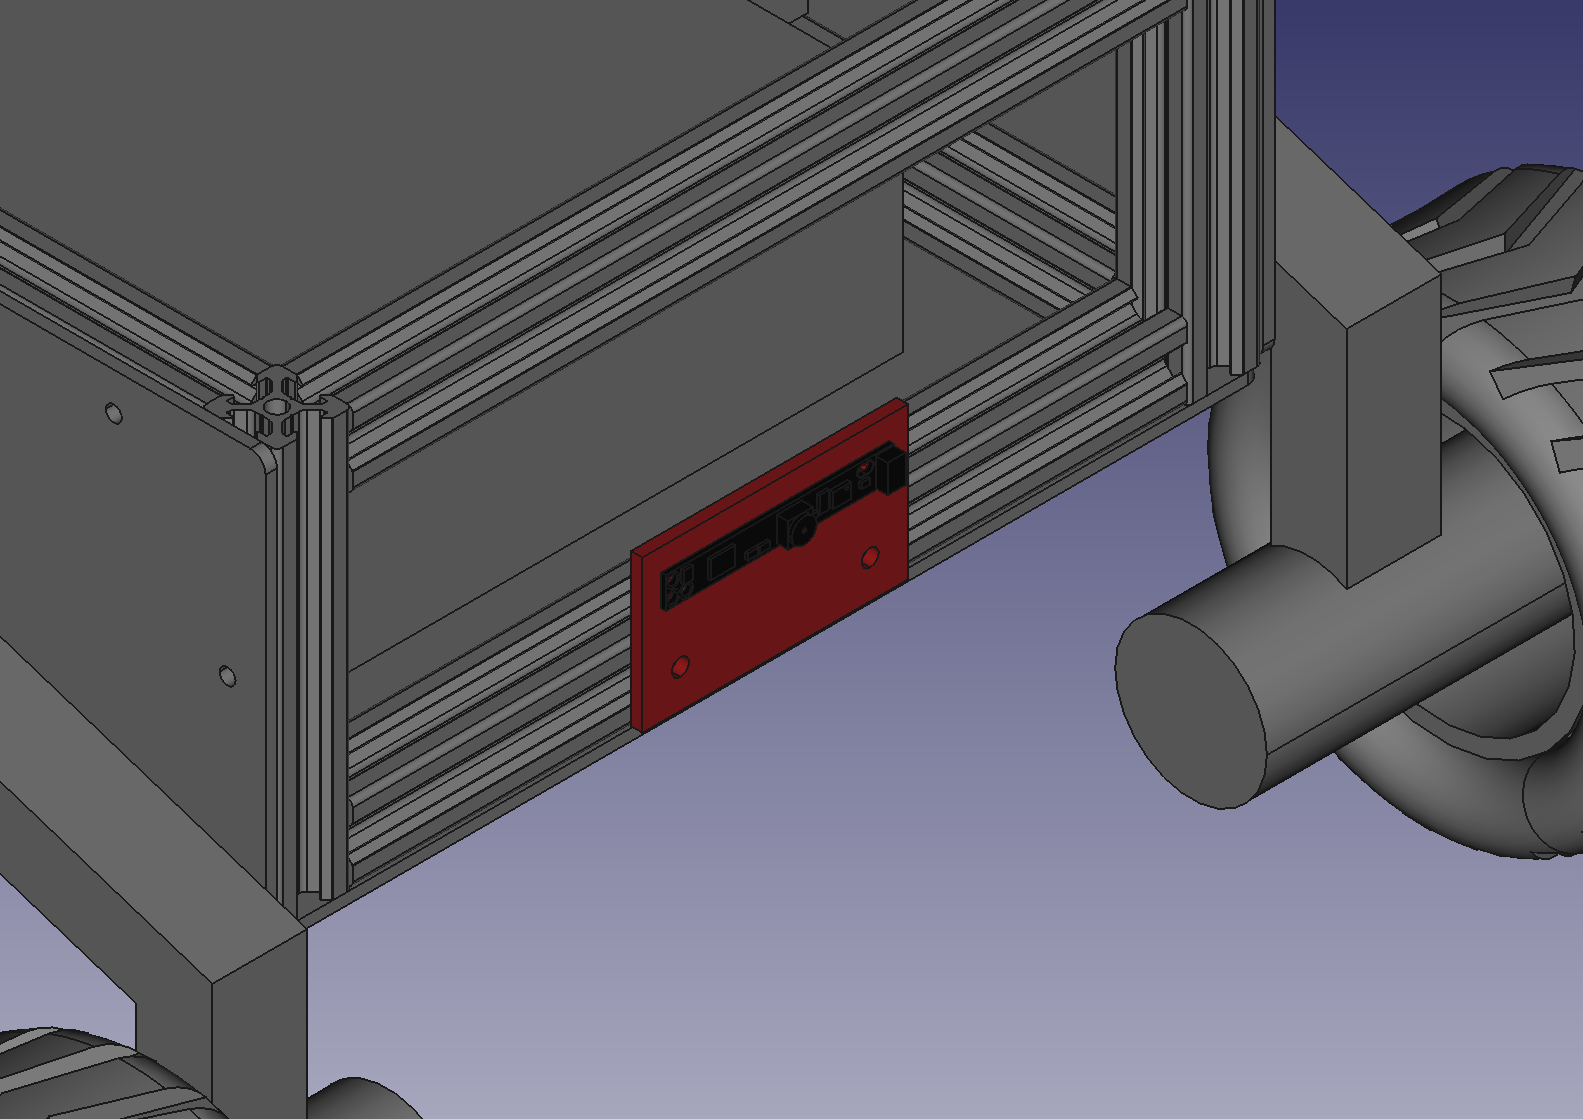
\includegraphics[width=\textwidth]{cameraholder}

% \begin{figure} \centering 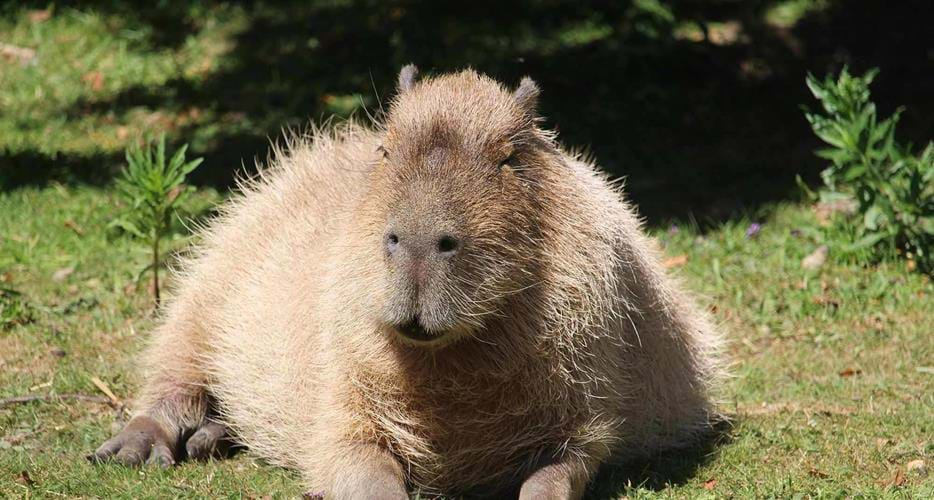
\includegraphics[width=0.9\textwidth]{capybara.jpg}
%     \caption{\label{fig:capybara}Капибара.} \end{figure}

\section{Сборка клешни}

Вставить ServoHolderRetainer в ServoHolder и закрепить их DIN-7985-M3 винтом
длиной 12 мм с гайкой DIN-934-M3.

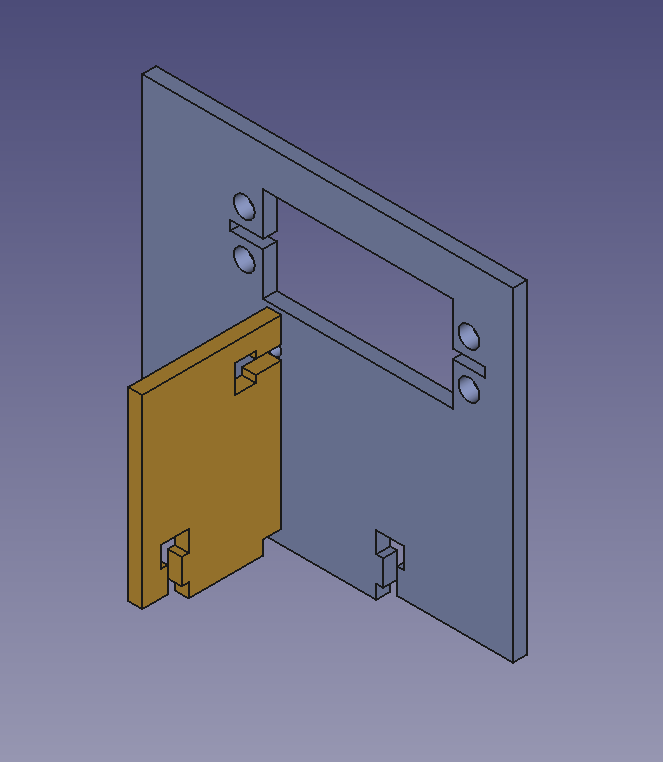
\includegraphics[width=\textwidth]{servoholder}

Вставить получившуюся конструкцию в TopPanel и закрептить DIN-7985-M3 винтами
длиной 12 мм с гайками DIN-934-M3.

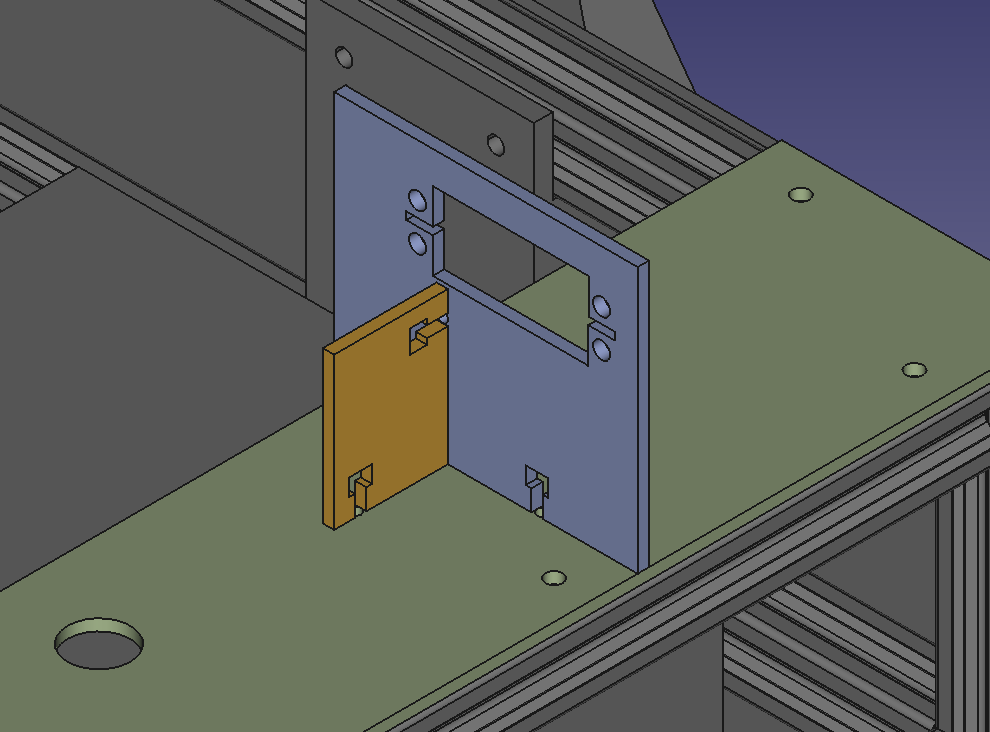
\includegraphics[width=\textwidth]{servoholder-toppanel}

Вставить сервопривод MG995 в ServoHolder так, чтобы вращающаяся часть была
направлена вправо и находилась ближе к переду робота (см. рисунок) и закрепить
его DIN-7985-M4 винтами длиной 8 мм с DIN-934-M4 гайками (гайки должны
находиться слева, чтобы винты не мешали движению клешни).

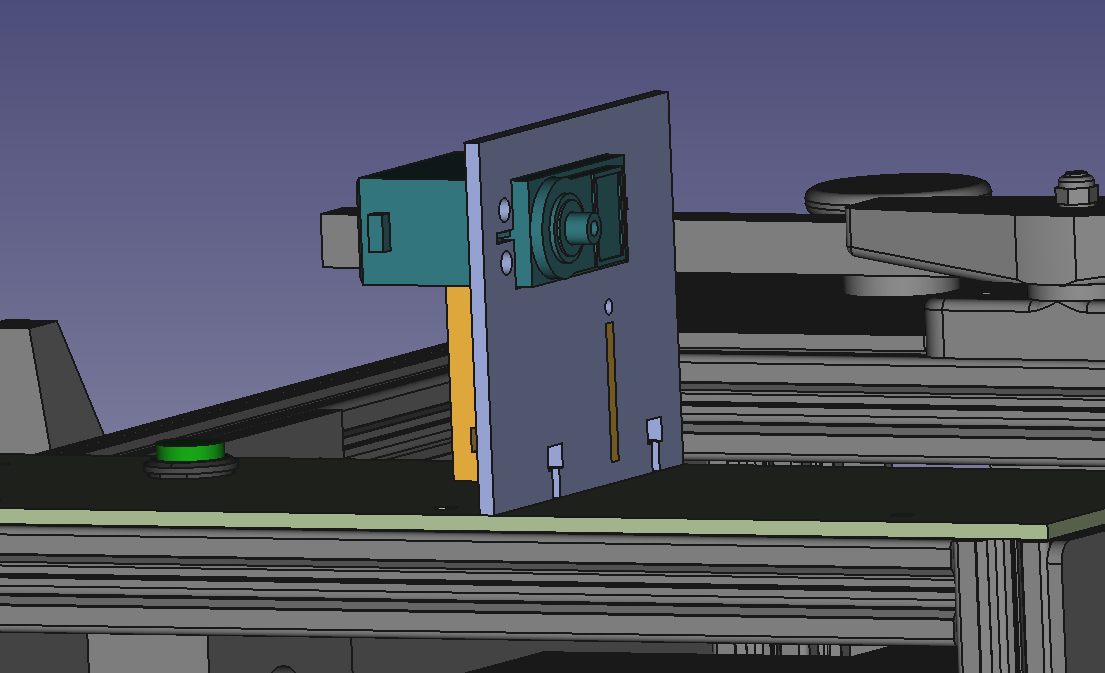
\includegraphics[width=\textwidth]{installedservo}

Прикрутить крестовую насадку сервопривода к Claw (клешне) 8 саморезами DIN-7986.

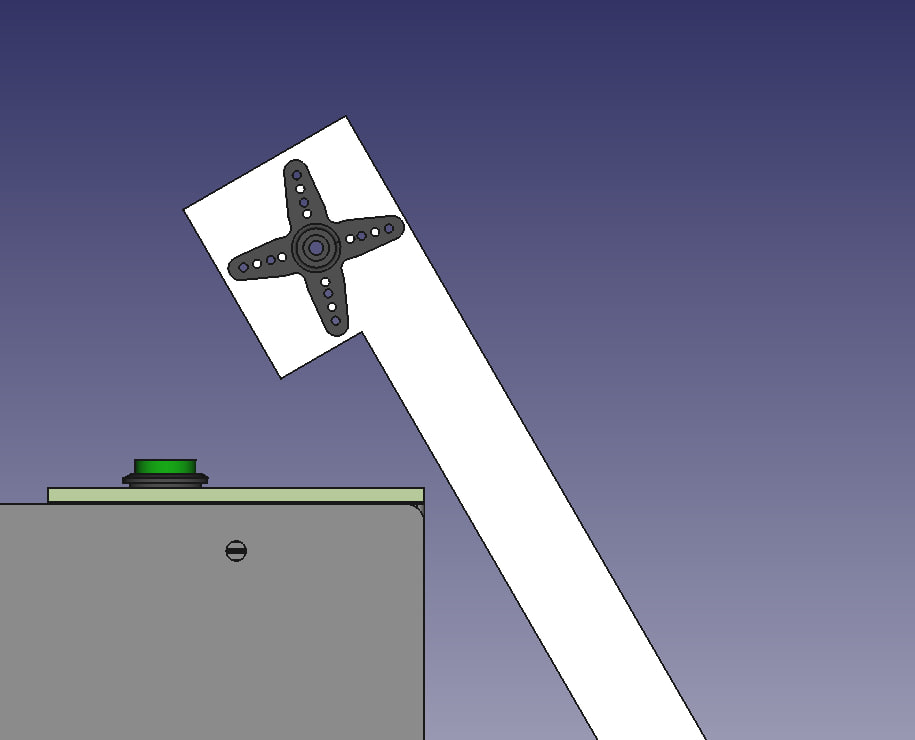
\includegraphics[width=\textwidth]{servo.png}

Повернуть сервопривод в крайнее положение против часовой стрелки (если руками
это сделать сложно, можно использовать какую-либо насадку).

Присоеденить клешню к сервоприводу так, чтобы в крайнем положении против часовой
стрелки сервопривода клешня была в нижнем положении (касалась верхней панели
робота).

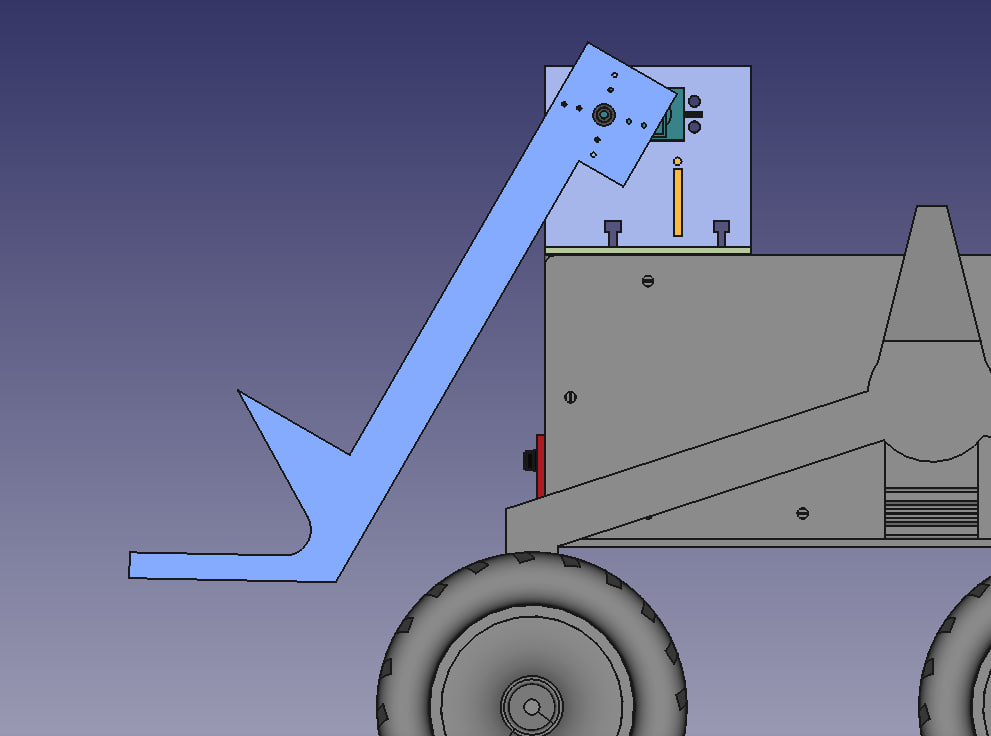
\includegraphics[width=\textwidth]{full_claw.png}

\end{document}
